\section{Discussion}
\label{sec:discussion}

%% FF(theta) dependance is probably tradeoff of FF factors listed near the top


%% for discussion

%% should include nested fits in Pe comparison plot
%% maybe 360 resonance is smeared out by dopants/impurities

% takeaway is assessment of Vbr between different methods is critical if enforcing Pe from independent measurement is goal
%% better parameterization

%% not sure how to organize % xx


%%%%%%%%%%%%%%%%%%%%%%%%%%%%%%%%%%%% -- %%%%%%%%%%%%%%%%%%%%%%%%%%%%%%%%%%%%
%% General fitting message
We have demonstrated that the many parameters of the PDE model can be constrained using combinations of relative optical measurements and absolute PDE. The model shows predictive power in extrapolating PDE to unmeasured wavelengths, angles, operational media and a subset of temperatures. Given the reliability of $n, k$ data in the visible-NIR and lack of structure, the extrapolation to dense media for modelling ExCT should be quite robust. The agreement between sequential and global fit methods indicate PDE for specific wavelengths may be modeled without full spectral information. % If only UV PDE is under study, $P_e(V)$ from PDE or rate-based measurements may be used; otherwise the PDE derived $P_e(V)$ is more accurate.
Including data below 350~nm should better constrain $dp^*$ regardless of fit method, and future work may investigate a `soft-edge' model with probabilistic charge collection between $0<z<dp^*$ which flattens the response about 360~nm.

%% data and liquid nobles
The model's underestimated LAr PDE emphasizes impact of oxide layer thickness and encourages further study of VUV optical constants at cryogenic temperatures. This is challenging as $\sio$ optical properties are known to vary with growth conditions and techniques \cite{sio2_properties1, sio2_properties2, SiO2_dep_2001_khodier}. Results from \cite{sio2_properties1} may be implemented in future work. The steep dispersion of liquid noble $n$ values near their scintillation response, and slope of \sio $n, k$ near 128~nm, underscores the importance of including spectral information in computation.%For LAr and LXe we have uncertainty in the exact value of $n$ at long wavelengths ($\lambda \sim 1000$~nm), and if the IR resonance used for the Sellmeier parameterization in \cite{lar_lxe_GRACE2017} is physical. In LXe the estimated range of values $n(1000\text{nm})=1.35-1.4$ only modifies the $\sim 80\%$ transmission into silicon by 1.2\%\footnote{1.35 taken from the pre-resonance region in \cite{lar_lxe_GRACE2017}, 1.4 from $n\approx \sqrt{\epsilon_r}$, $\epsilon_r=1.96$ reported in \cite{Aprile_2010}.}.

\subsection{Input Optical Datasets}
Although the Franta optical dataset can fit the PDE, results are rejected with limited confidence due to the poorer quality of fit and $P_h$ values higher than expectation from impact ionization ratios between electrons and holes\cite{gallina_avalanche_2019, mcintyre_avalanche_1973, oldham_avalanche}. The increased $P_h$ is not unexpected as the dataset describes ultrapure silicon, while SiPMs are heavily doped which increases photoabsorption \cite{photoAbs_doping_Abroug2008}. These results illustrates some quasi-degeneracy between photoabsorption data, junction size and $P_h$ in the NIR; PDE data extending to 1050~nm would help resolve this. Alternatively, direct study of $P_h$ could be achieved using a two-photon absorption technique \cite{Pape_2024} or by studying the rate of delayed crosstalk, which is expected to be entirely hole-driven in P-on-N devices. Given a known doping profile, implementation of the complete Franta optical model, which includes the impact of dopants on photoabsorption, would be possible.

\subsection{Angular Measurements}
We found the shadowing effect on the HPK-VUV4 essential to reproduce other angular measurements at $\sim 175$~nm (\autoref{fig:vuv4_reflectivity}). No shadowing was observed for the FBK device likely due to smaller or asymmetric resistors. At longer wavelengths the effective $FF(\lambda)$ can increase as the charge collection region is not uniform in depth\cite{ACERBI2018_FF}. We suspect the interplay between this effect and shadowing drives the measured increase of $FF(\theta)$ with wavelength.

For the FBK angular scans, the variation in oscillations (and oxide thickness) may be explained by surface thickness variations, as the beam's exact position varied between installs. Regardless, discrepancies in the FBK data highlighted the need for a more precise understanding of the experimental setup's optics, namely effects of the lamp's underlying spectrum and MC transfer function. As oscillations in equation \autoref{eq:transmission} are not symmetric with respect to $\theta$ or $\lambda$, the averaged transmission's maxima can shift depending on transfer function shape.

%% atp cmparison section
\subsection{Comparing Avalanche Triggering Probabilities} % xx
\label{sec:ATP}

The nested $P_e$ fits perform best and are less susceptible to bias from low-voltage data or inaccurate breakdown voltages. The exact mapping between rate-based or PDE driven $P_e(V)$ (3A vs 3B in \autoref{tab:fitting_procedure}) is difficult, requiring the absolute accuracy of UV transmission and $FF$. Additionally, the assumption of a sharp transition from $P_e$ to $P_h$ about $X_{PN}$ can allow longer wavelengths to bias PDE driven $P_e$. Fitting for the $V_e$ shape parameter is sensitive to the breakdown voltage, which can differ between IV or gain based analysis; our rate based measurements ($V_e = 1.5-1.8 \pm 0.1$) agree with PDE driven $V_e$ only if a shift in voltage is applied, which can be seen in the shifted dotted lines of \autoref{fig:Ph}. We suspect the low nested FBK $P_e$ values (purple squares in \autoref{fig:Ph}) are compensation for other overestimated terms; decreasing $FF=0.8\to0.7$ drives $P_e$ towards unity as expected.

The takeaway is that $PDE$ derived $P_e(V)$ should be used when calculating the absolute efficiency over many wavelengths. If studying voltage dependence in a narrow UV regime, especially in a relative measurement, either $P_e(V)$ value may be used. A $P_e$ parameterization function with two degrees of freedom may reduce the sensitivity to breakdown voltage or equivalently better describe lower voltage PDE. % For HPK, the shape of $PDE(V)$ and $P_e(V)$ curves also differ, likely due to a systematic difference between the $Q_A(V)$ correction and primary pulse identification method.

\begin{figure}[htbp]
\centering
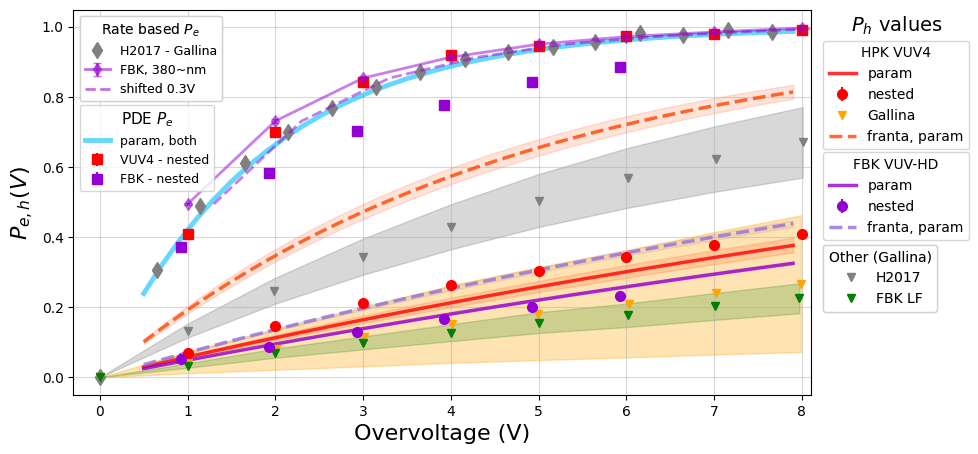
\includegraphics[width=.9\linewidth]{fig-ATP_comparison_v2.png}
\caption{\label{fig:Ph}
Comparison of avalanche probabilities. Upper curves are $P_e$ from fits or rate-based measurement. All parameterized fits give essentially the same $P_e$ curve (gray line). The unparameterized or `nested' $P_e$ values deviate slightly from the parameterization. Lower curves are $P_h$ values, taken from this work or \cite{gallina_avalanche_2019}. The Franta driven $P_h$ values are higher than the default dataset's due to the lower photoabsorption in the NIR and are less supported by other literature and physical expectation.}
\end{figure}

\autoref{fig:Ph} compares our various $P_h$, $P_e$ curves and those reported by Gallina \cite{gallina_avalanche_2019}. The similarity of the $P_e$ curves is remarkable, despite coming from different devices, optical data, measurement techniques and temperatures. The assumption that $P_e$ saturates to unity was validated for HPK. Further work should study the universality of $P_e$ between devices at temperatures below 160~K, and shape difference at low overvoltages. % The rate-based $P_e$ measurement is horizontally offset from the fit values. Allowing for a horizontal shift in voltage of 0.1~V, owing to uncertainty in breakdown voltage calculation between datasets, the curves are similar.
The $P_h$ curves have larger variance. The default-dataset derived $P_h$ values are low and fall within the large uncertainty bands of the VUV4 device from \cite{gallina_avalanche_2019}. Higher Franta-derived values are included, with the resulting VUV4 parameterization ($V_e = 4.7$) exceeding that of the H2017 device in \cite{gallina_avalanche_2019}. %$P_h$ between fits are in better agreement for the FBK device likely due to stronger constraint on $\tox$ from the oscillations.
A larger variance in $P_h$ across different devices is not unexpected at moderate overvoltages.%, as the lower mobility of holes prevents $P_h$ from quickly saturating.
The sharp transition at $X_{PN}$ assumption may contribute, as larger junctions can have a less-well defined singular $P_h$ value.
%This may explain the underestimation of the VUV4's PDE near 480~nm (where both $W_p, W_n > 0$).

\subsection{Temperature Dependence} % xx
Preliminary $P_e(V)$ measurements showed negligible temperature dependence between 160~K and 253~K. The PDE reported in \cite{gallina_performance_2022} at both 160~K and 300~K, once quantum yield is included, are similar to those measured here. The shape of LAr $PDE(V)$ from Pershing \cite{Pershing_2022_argonPDE} actually suggest lower $P_e$ at 90~K, assuming the quantum yield in \cite{Lewis_2025_qy} is monotonic in energy. Lower $P_e$ with temperature is possible due to carrier freezeout overcoming the increase in mobility, or measurement contamination by fluorescence, which would contribute $P_h$ and inflate reported PDE.

The third FBK angular campaign measured relative $PDE(\theta)$ at 213~K and 163~K, producing identical oscillation patterns at both temperatures. This suggests the surface optics, at least at 400 and 600~nm, are unperturbed by those temperatures. The parameterized temperature dependence of the photo-absorption appears reliable, although in the future we hope validate it on PDE data below the 440~nm limit from \cite{siBandgap_dmPaper}. Future work may include the effect of carrier freezeout; the complete temperature response of PDE below 100~K is complex and requires further modeling.

% \section{Optimizing PDE for Liquid Nobles and Quantum Sensing}
% \label{sec:maximize}
% For specific applications, we investigate the theoretical upper limit of PDE for P-on-N devices with the single $\sio$ layer surface model. This requires maximizing the fill factor $FF$, the optical transmission and achieving junction geometry such that avalanches are electron-driven ($W_p \rightarrow 1.0$). In this case the PDE is approximately $PDE_{max} \approx FF \cdot T_{max}\cdot W_p$, provided the devices can be operated with $P_e\rightarrow 1.0$ and correlated avalanches are tractable. Maximizing fill factor is a difficult fabrication challenge, driven by the need for a low field boundary around each SPAD, quenching resistors and isolating trenches. Backside-Illuminated (BSI) structures are a promising approach, reaching $FF$ values close to 100\% \cite{ninkovic_avalanche_2007}. Multilayer anti-reflective coatings can improve transmission in the UV \cite{uvMulti_Hamden2011} and achieve near-100\% transmission for visible light \cite{JIA_solarcells_broadband_2017, solar_multilayer_review, multilayer_2005}; however this includes increased cost, complexity and is outside the scope of our model.

% \begin{table}[ht!]
% \centering
% \caption{\label{tab:quantum} Optimized $\sio$ thickness and junction geometries for maximizing high PDE. Relevant geometries are given for achieving $W_p=0.9$. For UV wavelengths (liquid nobles) the depth of the electron collection region $dp^*$ is given. For longer wavelengths the junction center $X_{PN}$ is given. Similar transmissions can be obtained for multiple oxide thicknesses, only values below 1~$\um$ are reported.}
% \smallskip
% \renewcommand{\arraystretch}{1.3}  % Default is 1.0
% {\footnotesize
% \begin{tabular}{|c|c|c|c|c|}
% \hline
% \textbf{Application} & \textbf{{$\bm{\lambda}$ (nm)}} & \makecell{\textbf{Maximum}\\\textbf{transmission}} & \textbf{$\bm{\tox}$ (nm)} & \textbf{$\bm{dp^*}$ or $\bm{X_{PN}}$} \\
% \Xhline{3\arrayrulewidth}
% LAr in vacuum & 127 $\pm$ 10 & 0.44 & 4.7 & 0.6~nm \\ \hline
% LAr           & 127 $\pm$ 10 & 0.38 & 3.45 & 0.6~nm \\ \hline
% Xe-doped LAr  & 175 $\pm$ 10 & 0.46 & 17.3 & 0.5~nm \\ \hline
% LXe           & 175 $\pm$ 10 & 0.40 & 44 & 0.5~nm \\ \hline
% Xe in $\ce{CF_4}$ & 175 $\pm$ 10 & 0.47 & 17.2 & 0.5~nm \\ \hline
% TPB \cite{TPB_Francini_2013}, PEN \cite{PEN_Kuniak2019} in LAr & 430 $\pm$ 80 & 0.76 & 71 & \small{$X_{PN}=$~550~nm} \\
% \Xhline{3\arrayrulewidth}
% Diamond NV center \cite{childress_diamond_2013} & 532 & 0.89 & 91.3 & 1.7 $\um$ \\ \hline
% Sodium D-line & 589 & 0.91 & 101  & 3.3 $\um$ \\ \hline
% NV center (zero-phonon) \cite{NV_zerophonon} & 637 & 0.91 & 328  & 5.6 $\um$ \\ \hline
% Rubidium D1, D2 lines \cite{mottola_optical_2023} & 780, 795 & 0.93 & 410, 671 & 21, 27 $\um$ \\ \hline
% Satellite-Ground QKD \cite{liao_satellite--ground_2017} & 850 & 0.93 & 731  & 45 $\um$ \\
% \hline
% \end{tabular}
% } % end of font size
% \end{table}
% % This requires the correlated avalanches typically associated with higher overvoltages remain experimentally tractable.
% % Backside-Illuminated (BSI) and 3D integrated SPADs are promising approaches,

% In \autoref{tab:quantum} the upper half correspond physics applications with argon or xenon and the lower half is wavelengths relevant to qubit manipulation or free-space laser operation in satellite-to-ground quantum key distribution \cite{liao_satellite--ground_2017}. Oxide thicknesses are calculated by maximizing \autoref{eq:transmission} at normal incidence, and junction geometries calculated to achieve $90\%$ absorption. Liquid noble applications include the optical coupling of the medium and are convolved with the emission spectra in\cite{fuji_lxe_2015, LAr_width_2021_ettore}.%, which modifies transmission at the percent level.
% We note for LXe scintillation both devices characterized in this work achieve $iPDE\sim$90\% when operated at reasonable overvoltage.

% LAr PDE close to 35\% is possible if very thin oxide devices can be fabricated, as $\sio$ is strongly absorbing at 128~nm. This again highlights the importance of accurate VUV $k$ data. Notably, 6\% higher PDE can be achieved for Xe-doped LAr than pure LXe due to transmission enhancement via constructive interference. In $\ce{CF4}$, the SiPM operational medium of SBC\cite{sbc_snowmass2021}, the transmission of xenon light is $\sim 47\%$, a noticeable increase from vacuum\footnote{$n=1.24$ is taken for liquid $\ce{CF4}$ from \cite{index_cf4_chemPhys, index_cf4_french}}. For quantum applications transmission of $\sim$90\% is possible, combined with $W_p \approx 0.9$ gives PDE of $\sim$80\%. We anticipate future designs can push $FF$ close to unity while retaining high avalanche efficiency and timing resolution. Digital SiPMs may provide the best path forward for their insensitivity to correlated avalanches within a single SPAD \cite{Pratte_2021}. This discussion of course ignores the complexity of silicon doping and the engineering of suitable electric field profiles.

\section{Optimizing PDE for Liquid Nobles and Quantum Sensing}
\label{sec:maximize}

We estimate the theoretical upper limit of PDE for P-on-N devices using the single $\sio$ layer surface model. Maximizing PDE requires large fill factor $FF$, transmission, and junction geometries favoring electron-initiated avalanches ($W_p \sim 1$), assuming operation with $P_e(V) \sim 1$ while correlated avalanches remain tractable. The PDE becomes: $PDE_{\text{max}} \approx FF \cdot T_{\text{max}} \cdot W_p$.

Achieving high $FF$ remains fabrication-limited due to maintaining a low boundary field within each SPAD, quenching resistors, and isolation trenches. Backside-illuminated structures show promise for $FF \sim 100\%$ \cite{ninkovic_avalanche_2007}. Multilayer anti-reflective coatings enable near-unity transmission in the visible and improved UV performance \cite{uvMulti_Hamden2011, JIA_solarcells_broadband_2017, solar_multilayer_review, multilayer_2005}, though at increased cost and complexity outside this model's scope. \autoref{tab:quantum} lists optimized parameters for particle physics applications and qubit control, free-space quantum communication \cite{liao_satellite--ground_2017}. Oxide thicknesses maximize normal-incidence transmission, while junction geometries ensure $\sim90\%$ absorption.
\begin{table}[ht!]
\centering
\caption{\label{tab:quantum} Optimized $\sio$ thickness and junction geometries for maximizing PDE. Relevant geometries achieve $W_p=0.9$; for VUV wavelengths $dp^*$ is given and junction center $X_{PN}$ for others.}
\smallskip
\renewcommand{\arraystretch}{1.3}  % Default is 1.0
{\footnotesize
\begin{tabular}{|c|c|c|c|c|}
\hline
\textbf{Application} & \textbf{{$\bm{\lambda}$ (nm)}} & \makecell{\textbf{Maximum}\\\textbf{transmission}} & \textbf{$\bm{\tox}$ (nm)} & \textbf{$\bm{dp^*}$ or $\bm{X_{PN}}$} \\
\Xhline{3\arrayrulewidth}
LAr in vacuum & 127 $\pm$ 10 & 0.44 & 4.7 & 0.6~nm \\ \hline
LAr           & 127 $\pm$ 10 & 0.38 & 3.45 & 0.6~nm \\ \hline
Xe-doped LAr  & 175 $\pm$ 10 & 0.46 & 17.3 & 0.5~nm \\ \hline
LXe           & 175 $\pm$ 10 & 0.40 & 44 & 0.5~nm \\ \hline
Xe in $\ce{CF_4}$ & 175 $\pm$ 10 & 0.47 & 17.2 & 0.5~nm \\ \hline
TPB \cite{TPB_Francini_2013}, PEN \cite{PEN_Kuniak2019} in LAr & 430 $\pm$ 80 & 0.76 & 71 & \small{$X_{PN}=$~550~nm} \\
\Xhline{3\arrayrulewidth}
Diamond NV center \cite{childress_diamond_2013} & 532 & 0.89 & 91.3 & 1.7 $\um$ \\ \hline
Sodium D-line & 589 & 0.91 & 101  & 3.3 $\um$ \\ \hline
NV center (zero-phonon) \cite{NV_zerophonon} & 637 & 0.91 & 328  & 5.6 $\um$ \\ \hline
Rubidium D1, D2 lines \cite{mottola_optical_2023} & 780, 795 & 0.93 & 410, 671 & 21, 27 $\um$ \\ \hline
Satellite-Ground QKD \cite{liao_satellite--ground_2017} & 850 & 0.93 & 731  & 45 $\um$ \\
\hline
\end{tabular}
} % end of font size
\end{table}

For LXe scintillation both devices studied achieve $iPDE \sim 90\%$. In LAr, PDE approaching $\sim35\%$ is possible for very thin oxides. Xe-doped LAr can achieve $\sim6\%$ higher PDE than pure LXe by via constructive interference. In $\ce{CF4}$, the operational medium of SBC\cite{sbc_snowmass2021}, the transmission of xenon light is noticeably higher than in vacuum\footnote{$n=1.24$ is taken for liquid $\ce{CF4}$ from \cite{index_cf4_chemPhys, index_cf4_french}}. In quantum-sensing, transmission near $90\%$ combined with $W_p \approx 0.9$ implies PDE approaching $80\%$, given $FF \sim 100\%$. Digital SiPMs may provide the best path forward due to insensitivity to correlated avalanches \cite{Pratte_2021}. This analysis ignores the complexity of doping and engineering suitable electric-field profiles.